\chapter{Add a Chapter Title Here if you Wish}



Pellentesque porttitor, velit lacinia egestas auctor, diam eros tempus arcu, nec vulputate augue magna vel risus. Cras non magna vel ante adipiscing rhoncus. Vivamus a mi. Morbi neque. Aliquam erat volutpat. Integer ultrices lobortis eros. Rosa Olin Jackson~\cite{waveshaping} ad litora torquent per conubia nostra.\par

Pellentesque habitant morbi tristique senectus et netus et malesuada fames ac turpis egestas. Proin semper, ante vitae sollicitudin posuere, metus quam iaculis nibh, vitae scelerisque nunc massa eget pede. Sed velit urna, interdum vel, ultricies vel, faucibus at, quam. Donec elit est, consectetuer eget, consequat quis, tempus quis, wisi. In in nunc. Class aptent taciti sociosqu ad litora torquent per conubia nostra, per inceptos hymenaeos.\par



% To remove the numeric value of the subheading below, insert an asterisk after \section (i.e., \section*)

\section{Chapter 1 Heading 3 (subheading)}

\begin{figure}
%Use the scale parameter to size the image
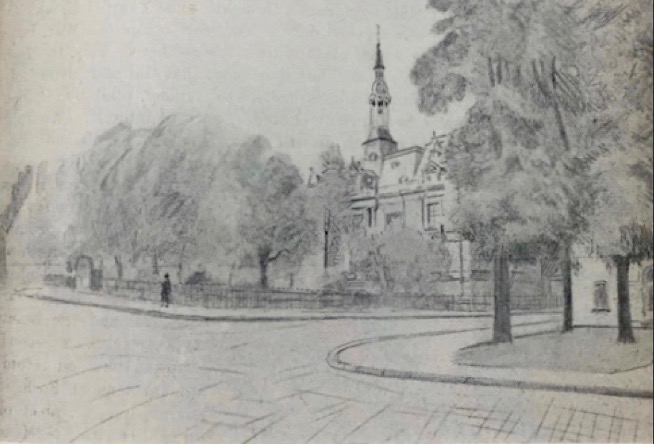
\includegraphics[width=1\textwidth]{figures/Picture1}

% here is an alternate way to scale images based on specific sizes
%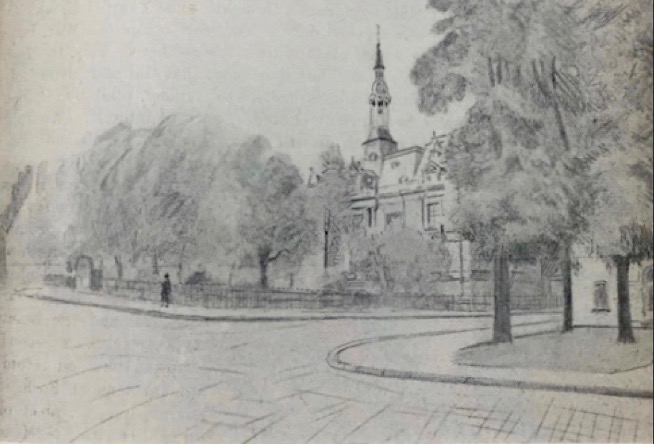
\includegraphics[width=5cm, height=4cm]{figures/Picture1}
\label{fig:img1}
\caption{Example of a basic figure title}
\end{figure}

Note that every figure present in the document should be referenced from somewhere within the text.  This is an example of a reference to a figure in the thesis: see Fig.~\ref{fig:img1}. 


Cras faucibus condimentum odio. Sed ac ligula. Aliquam at eros. Etiam at ligula et tellus ullamcorper ultrices. In fermentum, lorem non cursus porttitor, diam urna accumsan lacus, sed interdum wisi nibh nec nisl. Ut tincidunt volutpat urna. Mauris eleifend nulla eget mauris. Sed cursus quam id felis. Curabitur posuere quam vel nibh. Cras dapibus dapibus nisl.\par

Vestibulum quis dolor a felis congue vehicula. Maecenas pede purus, tristique ac, tempus eget, egestas quis, mauris. Curabitur non eros. Nullam hendrerit bibendum justo. Fusce iaculis, est quis lacinia pretium, pede metus molestie lacus, at gravida wisi ante at libero. Quisque ornare placerat risus. Ut molestie magna at mi. Integer aliquet mauris et nibh. Ut mattis ligula posuere velit. Nunc sagittis.\par

\subsection{\emph{Chapter 1 Heading 4 (Sub-heading)}}

Curabitur varius fringilla nisl. Duis pretium mi euismod erat. Maecenas id augue. Nam vulputate. Duis a quam non neque lobortis malesuada. Praesent euismod. Donec nulla augue, venenatis scelerisque, dapibus a, consequat at, leo. Pellentesque libero lectus, tristique ac, consectetuer sit amet, imperdiet ut, justo. Sed aliquam odio vitae tortor. Proin hendrerit tempus arcu. In hac habitasse platea dictumst. Suspendisse potenti.\par
